
\begin{table*}[t!]
	\centering
	\small
	\resizebox{0.99\textwidth}{!}{
		\begin{tabular}{ccccccccc}
            \toprule
            \multirow{2}{*}{\textbf{Category}} & \multirow{2}{*}{\textbf{Model}} & \multirow{2}{*}{\textbf{Context Length}} & \multicolumn{6}{c}{\textbf{Answer Prediction (F1)}} \\
            \cmidrule(lr){4-9} & & & Single Hop & Multi Hop & Temporal & Open Domain &  Adversarial & \textbf{Overall}\\
            \midrule
                \rowcolor{blue!20} Human & Human & -  & 95.1 & 85.8 & 92.6 & 75.4 & 89.4 & 87.9  \\
            \midrule
                \multirow{4}{*}{Base} & \texttt{Mistral-Instruct-7B} & 8K  & 10.2 & 12.8 & 16.1 & 19.5 & 17.0 & 13.9 \\
                & \texttt{Llama-2-Chat-70B} & 4,096  & 19.7 & 14.4 & 13.3 & 15.9 & 22.1 & 17.9 \\
                & \texttt{GPT-3.5-turbo} & 4,096  & \textbf{29.9} & 23.3 & \textbf{17.5} & \textbf{29.5} & 12.8 & 22.4 \\
                & \texttt{GPT-4-turbo} & 4,096  & 23.4 & \textbf{23.4} & 10.4 & 24.6 & \textbf{70.2} & \textbf{32.1} \\

            \midrule
                \multirow{4}{*}{Long context} & \multirow{4}{*}{\texttt{GPT-3.5-turbo-16K}} & \cellcolor{gray!25} 4K  & 31.7 & 25.4 & 16.8 & 27.6 & \textbf{13.1} & 24.1  \\
                 & & \cellcolor{gray!40} 8K  & 38.8 & 31.2 & 21.0 & 35.0 & 8.4 & 25.2  \\
                 & & \cellcolor{gray!60} 12K  & 51.1 & 40.4 & \textbf{25.0} & 36.5 & 6.4 & 33.5  \\
                 & & \cellcolor{gray!75} 16K  & \textbf{56.4} & \textbf{42.0} & 20.3 & \textbf{37.2} & 2.1 & \textbf{37.8}  \\
            \bottomrule
        \end{tabular}
	}
 \vspace{-5pt}
        \caption{\textbf{Question answering performance} of \texttt{Base} and \texttt{Long-context} models. Optimal performance is in \textbf{bold}. Results are based on F1-score for answer prediction; higher is better.}
	\label{tab:qa_results}
\end{table*}



\begin{table*}[t!]
	\centering
	\small
	\resizebox{0.99\textwidth}{!}{
		\begin{tabular}{P{0.7in}P{0.2in}P{0.4in}P{0.4in}P{0.4in}P{0.5in}P{0.4in}P{0.5in}P{0.5in}P{0.5in}P{0.5in}P{0.5in}P{0.5in}P{0.5in}}
            \toprule
              &  &  \multicolumn{6}{c}{\textbf{Answer Prediction (F1 score)}} &
             & \multicolumn{5}{c}{\textbf{Recall Accuracy (R@$k$)}} \\
            \cmidrule(lr){3-8} \cmidrule(lr){9-14} \multirow{2}{*}{\textbf{Retrieval Unit}} & \multirow{2}{*}{\textbf{top-$k$}} & Single Hop & Multi Hop & Temporal & Open \newline Domain &  Adver-\newline -sarial & \textbf{Overall} & Single Hop & Multi Hop & Temporal & Open \newline Domain &  Adver- \newline -sarial & \textbf{Overall} \\
            \midrule
            \texttt{None} & -  & 29.9 & 23.3 & 17.5 & 29.5 & 12.8 & 22.4 & - & - & - & - & - & -  \\
            \midrule
                 \multirow{4}{*}{\texttt{Dialog}} & \cellcolor{gray!30} 5 & 42.9  & 19.4  & 21.3  & 35.8  & 31.9  & 31.7  & 
                 66.2  & 34.4 &  89.2 & 38.5 & 45.7 & 58.8  \\
                 & \cellcolor{gray!45} 10 & 46.3  & 26.8  & 24.8  & 37.5  & \textbf{29.8} & 34.6  & 72.8 & 247.4 &  97.3 & 53.8 &  54.3 & 67.5 \\
                 & \cellcolor{gray!60} 25 & 48.1 & 36.1 & \textbf{26.2} & \textbf{43.4} & 23.4 & \textbf{35.8} & 87.5 & 64.1 & \textbf{97.3} &  \textbf{67.9} & 69.1 & 79.9 \\
                 & \cellcolor{gray!75} 50 & \textbf{50.9} & \textbf{37.2} & 24.6 & 38.3 & 17.0 & 34.8 &  \textbf{90.4} &  \textbf{75.5} &  97.3 &  67.9 &  \textbf{77.7} &  \textbf{84.8} \\
            \midrule
                \multirow{4}{*}{\texttt{Observation}} & \cellcolor{gray!30} 5 &  44.3  & 30.6  & 41.9  & 40.2  & \textbf{44.7}  & \textbf{41.4}  &   52.9 &  40.1 &  81.1 &  38.5 &  29.8 & 49.6 \\
                & \cellcolor{gray!45} 10 & 42.2  & 30.5  & \textbf{42.1}  & 41.9  & 36.2  & 38.8  &  57.4 &  53.1 &  \textbf{83.8} & 46.2 &  41.5 &  57.1\\
                & \cellcolor{gray!60} 25 & \textbf{44.6}  & 33.2  & 41.8  & 41.9  & 27.7  & 38.0  & \textbf{71.3} &  63.8 &  83.8 &  66.7 &  45.7 & 66.0 \\
                & \cellcolor{gray!75} 50 & 44.0  & \textbf{34.5}  & 41.1  & \textbf{41.9}  & 27.7  & 37.8  &  72.8 &  \textbf{73.2} &  83.8 &  \textbf{74.4} &  \textbf{56.4} &  \textbf{71.1}\\
            \midrule
                \multirow{4}{*}{\texttt{Summary}} & \cellcolor{gray!30} 2 &  34.6  & 15.7  & 26.9  & 26.5  & 36.2  & 29.9  &   68.4 &  39.6 &  56.8 & 50.0 & 73.4 &  61.5 \\
                & \cellcolor{gray!50} 5 & \textbf{36.6}  & \textbf{16.6} & \textbf{31.0} & \textbf{34.7}  & 38.3  & \textbf{32.5} &   81.6 &  57.0 &  70.3 &  60.3 &  86.2 &  75.1 \\
                & \cellcolor{gray!70} 10 & 34.5 & 14.7  & 29.3  & 31.6  & \textbf{40.4}  & 31.5  &  \textbf{93.4} &  \textbf{82.3} &  \textbf{91.9} &  \textbf{80.8} &  \textbf{94.7} &  \textbf{90.7} \\
            \bottomrule
        \end{tabular}
	}
 \vspace{-5pt}
        \caption{\textbf{Question answering performance} of RAG-based \texttt{GPT-3.5-turbo-16k}.  Optimal performance is in \textbf{bold}. Results are based on F1-score metric for answer prediction and recall@$k$ for recall accuracy; higher is better.}
	\label{tab:qa_rag_results}
 \vspace{-10pt}
\end{table*}

\section{Experimental Results}



We evaluate and analyze the comprehensive performance of all baseline methods for question answering (\Sref{ssec:qa-results}), event graph summarization (\Sref{ssec:event-results}), and multi-modal dialogue generation (\Sref{ssec:dialog-results}).

\subsection{Question Answering Task}
\label{ssec:qa-results}


Tables~\ref{tab:qa_results} and~\ref{tab:qa_rag_results} present the performance results for the question answering task. We find that:
\textbf{(1) LLMs with limited context length face challenges in understanding extremely long conversations} due to truncated context windows. Despite \texttt{gpt-4-turbo} emerging as the top-performing model with an overall score of 32.4, it notably lags behind the human benchmark of 87.9;
\textbf{(2) long-context LLMs can comprehend longer narratives, yet they are prone to generating hallucinations}. \texttt{gpt-3.5-turbo-16k} outperforms other approaches, but its performance on adversarial questions drops to a mere 2.1\%, as compared to 22.1\% using \texttt{Llama-2-Chat} and 70.2\% using \texttt{GPT-4-turbo} with 4K context windows. This indicates that LLMs can be easily misled into generating hallucinations when they are subjected to long contexts;
\textbf{(3) RAG is effective when conversations are stored as observations}. There is a noticeable 5\% improvement with \texttt{gpt-3.5-turbo} when the input is top 5 relevant observations instead of pure conversation logs. This improvement falters with an increase in the number of retrieved observations, suggesting that it is important to reduce the signal-to-noise (SNR) ratio in retrieved contexts for models to utilize the context accurately. Conversely, using session summaries as context does not significantly improve the performance despite high recall accuracies\footnote{For summary-based RAG models, the recall accuracy is based on retrieving the summary of the relevant session(s).}, likely due to loss of information during the conversion of dialogs to summaries.

The interesting finding is that \textbf{time reasoning and open-domain knowledge questions are the most challenging scenarios}.

(1) LLMs face challenges in understanding time concepts within dialogues, which is consistent with findings from other single-turn-based benchmarks focused on temporal reasoning capabilities for LLMs~\cite{wang2023tram}.

(2) LLMs struggle with open-domain knowledge and degrade in the RAG setting. This suggests that while certain open-domain knowledge may be embedded within the model's parameters, introducing improper context from inaccurate retrieval can lead to a decline in performance~\cite{mallen-etal-2023-trust}.


\begin{table*}[t!]
	\centering
	\small
	\resizebox{0.99\textwidth}{!}{
		\begin{tabular}{cccccccccc}
            \toprule
            \multirow{2}{*}{\textbf{Category}} & \multirow{2}{*}{\textbf{Model}} & \multirow{2}{*}{\textbf{Context Length}} & \multicolumn{3}{c}{\textbf{ROGUE}} & \multicolumn{3}{c}{\textbf{FactScore}} \\
            \cmidrule(lr){4-6} \cmidrule(lr){7-9} & & & \textbf{ROGUE-1} & \textbf{ROGUE-2} & \textbf{ROGUE-L} & \textbf{Precision} & \textbf{Recall} & \textbf{F1} \\
            \midrule
                \multirow{4}{*}{Base} & \texttt{Mistral-Instruct-7B} & 8K & 29.4 & 7.2 & 14.1 & 27.1 & 19.8 & 23.0 \\
                & \texttt{Llama-2-Chat-70B} & 4,096 & 28.1 & 9.3 & 14.8 & 36.3 & 22.7 & 28.3 \\
                & \texttt{GPT-4-turbo} & 4,096 & 38.8 & 11.4 & 20.6 & \textbf{51.6} & 41.8 & 45.1 \\
                & \texttt{GPT-3.5-turbo} & 4,096 & \textbf{41.1} & \textbf{13.5} & \textbf{20.9} & 45.3 & \textbf{46.5} & \textbf{45.9} \\
            \midrule
                Long context & \texttt{GPT-3.5-turbo-16K} & 16K & 36.2 & 8.5 & 16.4 & 42.3 & 37.8 & 39.9  \\
            \bottomrule
        \end{tabular}
	}
 \vspace{-1pt}
        \caption{\textbf{Event summarization performance} of \texttt{Base} and \texttt{Long-context} models. The optimal performance is shown in \textbf{bold}. Results are based on ROUGE and FactScore \cite{min2023factscore} metrics; higher is better.}
	\label{tab:summ_results}
\end{table*}

\begin{figure*}[t]
    \centering
    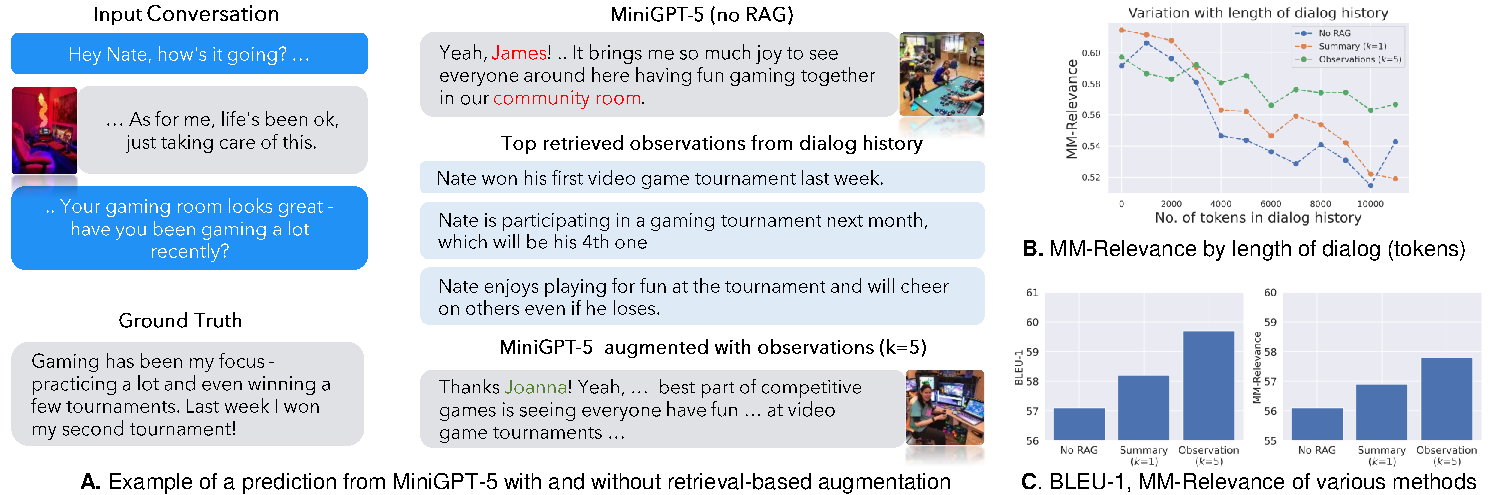
\includegraphics[width=0.99\textwidth]{figures/minigpt5_results.pdf}
    \vspace{-1pt}
    \caption{\textbf{Multimodal dialog generation performance of MiniGPT-5}. (A) an example of multimodal dialog predicted using MiniGPT5 with and without observation as retrieved context, (B) Variation of MM-Relevance score with length of dialog history, and (C) comparison of RAG-based MiniGPT-5 methods.\label{fig:minigpt5}}
    \vspace{-1pt}
\end{figure*}




\subsection{Event Summarization Task}
\label{ssec:event-results}

Table~\ref{tab:summ_results} presents results for the event summarization task. The use of incremental summarization with \textbf{\texttt{gpt-3.5-turbo} leads to the highest performance} in both recall and F1 score. While \texttt{gpt-4-turbo} records a 5.3\% improvement in precision over with \texttt{gpt-3.5-turbo}, it does not fare as well in terms of recall. The event summarization task requires long-range dependency to understand the temporal and causal connections between the events discussed by the speaker in multiple sessions (see Figure~\ref{fig:temporal-event}). Contrary to expectations, the \textbf{long-context model does not surpass the base model}, despite its capability for extended-range reasoning facilitated by a larger context window. \texttt{gpt-3.5-turbo-16k} exhibits a decline in both precision (by 3.0\%) and recall (by 8.7\%) compared to \texttt{gpt-3.5-turbo} which has a 4K context window. This suggests that \textbf{long-context models may not be proficient at utilizing their context appropriately}, which also aligns with similar findings in \citet{li2023loogle} as well as the QA task in \dataset{}. In terms of both the ROUGE and FactScore metrics, commercial models (\texttt{gpt-4-turbo}, \texttt{gpt-3.5-turbo}) significantly outshine their open-source counterparts. Nonetheless, there remains considerable scope for improving performance on this task.

From a manual analysis of predicted summaries, we identify five broad categories of event summarization errors made by LLMs: (1) \textbf{missing information} in events because the model fails to make temporal and/or causal connections over a lengthy conversation; (2) \textbf{hallucinations} i.e., models pad extra details that are either not present in the conversation or are part of a different event in the same session; (3) errors from \textbf{misunderstanding of dialog cues} such as humor or sarcasm is a distinctive issue with comprehension of dialogs; (4) inaccurate \textbf{speaker attributions}; and (5) insignificant dialogs that are wrongly considered as \textbf{salient} events. See examples in Table~\ref{tab:summary_errors} in the Appendix.



\subsection{Multi-Modal Dialog Generation Task}
\label{ssec:dialog-results}

Figure~\ref{fig:minigpt5} illustrates the effectiveness of various MiniGPT-5 training variants in multi-modal dialogue generation. Incorporating context into training enhances performance, with the inclusion of observation as context yielding significantly improved results. For instance, in Figure~\ref{fig:minigpt5}A, the retrieved observations contain information about the speaker's experience in video game tournaments, which leads to the prediction of dialog and images that are more faithful to the speaker's persona.
This observation is consistent with earlier findings from the QA task as well (see Table~\ref{tab:qa_rag_results}). Also, we observe that the MM-Relevance score drops with an increase in the length of dialog history (see Figure~\ref{fig:minigpt5}B). Retrieval-augmented generation alleviates the drop in MM-Relevance to some extent. 
